\documentclass[12pt,a4paper]{article}


\usepackage[left=2.5cm, right=2.5cm, top=3cm, bottom=3cm]{geometry}
\usepackage{amsmath, amsthm, amssymb}
\usepackage{hyperref}
\usepackage{graphicx}
\usepackage{url}

\begin{document}

\title{\Huge \bf Moogle!}
\author{\LARGE Luis Daniel Silva Martínez \\ C-111}
\date{21 de Julio, 2023}
\maketitle

\vspace{1cm}
\begin{figure}[h]
    \center
    
\includegraphics[width=4cm]{matcom.jpg}
\end{figure}


\begin{figure}[h]
    \center
    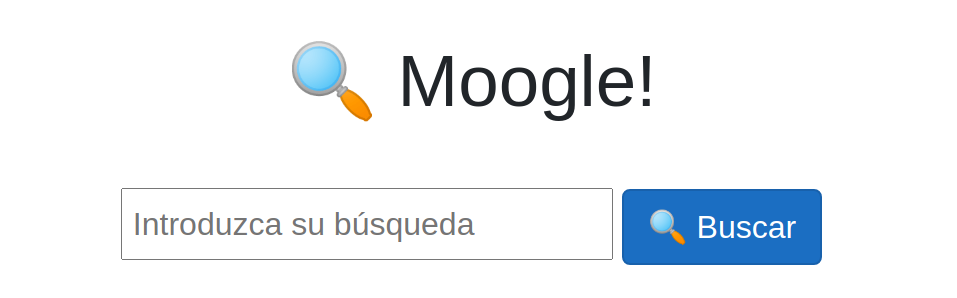
\includegraphics[width=15cm]{moogle.png}
\end{figure}



\newpage
\tableofcontents
\newpage


\section{Introducción}\label{sec:intro}
¿Alguna vez ha deseado buscar entre todos sus archivos de texto una palabra o frase particular? ¿Ha deseado organizar sus documentos de texto según su relevancia respecto a una búsqueda? 
Pues usted debería probar Moogle!, el nuevo buscador de texto actualmente sensación entre decenas de estudiantes de la Facultad de Matemáticas y Computación de la Universidad de La Habana.
\subsection{Qué es Moogle!?}\label{sub:what}
Moogle! es una aplicación totalmente original desarrollada con tecnología .NET Core 6.0, específicamente usando Blazor como framework web para la interfaz gráfica, y en el lenguaje C\#.
\subsection{Para qué sirve?}\label{sub:why}
Aplicando el Modelo Vectorial y la medida numérica TF-IDF, esta aplicación es capaz de leer 
archivos de texto en formato .txt ubicados en la carpeta Content y una búsqueda introducida por el usuario, y
devolver los documentos de texto relevantes en relación a lo buscado, 
ordenados de más relevantes a menos.
\subsection{Cómo usarlo?}\label{sub:how}
Para ejecutar el proyecto en Linux se debe abrir la terminal de Linux y ejecutar el comando:
\texttt{make dev}\\
En Windows, el comando para ejecutar la aplicación es (desde la carpeta raíz del proyecto):
\texttt{dotnet watch run --project MoogleServer}\\
Una vez con el proyecto andando, basta con escribir la búsqueda que se desea
realizar y pulsar el botón \textit{Buscar} para obtener los resultados.


\section{Funcionamiento}\label{sec:func}
La aplicación está dividida en dos componentes fundamentales:
\begin{itemize}
    \item \texttt{MoogleServer} es un servidor web que renderiza la interfaz gráfica y sirve los resultados.
    \item \texttt{MoogleEngine} es una biblioteca de clases donde está implementada la lógica del algoritmo de búsqueda.
\end{itemize}
\subsection{Implementación}\label{sub:impl}
El programa hace uso de un modelo vectorial con el algoritmo TF-IDF (Term Frequency - Inverse Document Frecuency)(\ref{equ:tfidf}).
Se separan todos los términos del texto en cada documento de la carpeta Content y se calcula
su valor TF-IDF para vectorizar los documentos. La entrada del usuario (query)
es tratada como un documento más, que recibe el mismo tratamiento anterior. Luego se compara el vector de la query con cada
vector de los documentos procesados usando la similitud de coseno(\ref{equ:simcos}) para obtener los archivos con
mayor semejanza a la búsqueda del usuario. Luego de obtener los resultados, en caso de recibir pocos, se calculará una sugerencia
de query usando la distancia de Leveshtein, bastante útil en casos donde ocurren errores de ortografía o typos.

\begin{equation}\label{equ:tfidf}
    TFIDF_{(t,d)} = \frac{tf}{tw} \times (\log_2\frac{1+N}{1+df})
\end{equation}
\begin{itemize}
    \item \emph{t}: término
    \item \emph{d}: documento
    \item \emph{tf}: frecuencia del término \emph{t} en \emph{d}
    \item \emph{tw}: total de términos en el documento \emph{d}
    \item \emph{df}: cantidad de documentos que contienen a \emph{t}
    \item \emph{N}: total de documentos en el corpus
\end{itemize}
\begin{equation}\label{equ:simcos}
    SimCos(\theta) = \frac{D \cdot Q}{||D|| \cdot ||Q||}
\end{equation}
\begin{itemize}
    \item D: vector del documento
    \item Q: vector de la query (búsqueda)
\end{itemize}


\subsection{Flujo}\label{sub:flow}
El proyecto sigue un camino marcado:
\begin{enumerate}
    \item Inicialización de la interfaz gráfica
    \item Procesamiento de los documentos de la carpeta Content
    \item Cálculo de los pesos TF-IDF de cada término en los documentos procesados
    \item Recepción de la búsqueda (query) introducida por el usuario
    \item Procesamiento de la query y cálculo del peso TF-IDF de cada término de la misma
    \item Cálculo de la similitud y relevancia de cada documento respecto a la query
    \item Obtención de un fragmento del documento (snippet) relevante respecto a la query
    \item Cálculo de una sugerencia en caso de que la búsqueda genere pocos resultados 
    \item Obtención de los resultados y mostrarlos en la interfaz gráfica
    \item Nueva búsqueda
\end{enumerate}

\subsection{Descripción del Código}\label{sub:code}
La lógica del algoritmo de búsqueda está implementada en el \texttt{MoogleEngine} con diferentes
clases.
\subsubsection{Moogle.cs}
La clase Moogle.cs es el puente entre todo lo que sucede por detrás en el proyecto y la interfaz gráfica
y la que se encarga de mantener el flujo del programa.
\subsubsection{DataBase.cs}
DataBase.cs se encarga de la obtención de los documentos en la carpeta Content y su tokenización usando Regex.
\subsubsection{TFIDF.cs}
Como su nombre lo indica, esta clase calcula el peso TFIDF de cada término y los asocia juntos.
\subsubsection{Query.cs}
la clase Query.cs toma la entrada del usuario, la tokeniza y calcula el TFIDF de los términos.
\subsubsection{Similarity.cs}
Similarity.cs calcula el score de cada documento respecto a la query con la fórmula de similitud del coseno para obtener los documentos más relevante
a la búsqueda. Además calcula el snippet que será mostrado junto al título del archivo de texto.
\subsubsection{Suggestion.cs}
Encargada de obtener una nueva query similar a la del usuario pero con terminos presentes en el corpus de documentos, usando el algoritmo de distancia de Leveshtein.


\section{Especificaciones}\label{sec:concl}
El programa está cableado para encontrar la carpeta Content dentro
de la carpeta que contiene a todo el proyecto. Para realizar búsquedas
entre los documentos .txt de su elección, deberá copiarlos a la carpeta
Content ubicada en el directorio principal del proyecto.
Moogle! puede demorarse cargando la interfaz gráfica en algunas máquinas,
y en su primera búsqueda tarda más de lo usual, cargando y procesando los
documentos en Content. Una vez realizada la primera búsqueda y cargados
los documentos, las siguientes búsquedas serán más rápidas.

\section{Funciones extras}\label{sec:extra}
\begin{itemize}
    \item Para introducir la query puede presionar Enter luego de escribir para que haga la búsqueda sin tocar el botón de Buscar.
    \item Para introducir la sugerencia dada por el programa puede presionarla directamente y llevara a cabo la búsqueda con esa sugerencia como query. 
     
\end{itemize}

\end{document}